\documentclass{beamer}

\beamertemplatenavigationsymbolsempty
\setbeamertemplate{footline}[frame number]

\usepackage{tikz}
\usetikzlibrary{matrix,positioning,arrows.meta,arrows,calc}

\title[Crisis]
{Decentralised location verification system}
\author{Conor Taylor}
\date{
	B.A.(Mod.) Computer Science\\
	Final Year Project, April 2016\\
	Supervisor: Stephen Barrett
}

\begin{document}

	\frame{\titlepage}
	
	\begin{frame}
    	\frametitle{Problem}
    	A system that allows participants to verify a users claimed location.
    	\\
    	\null
    	\visible<2->{
    		Goals:
   			\begin{itemize}
    			\item<3-> False location claims must be detectable.
    			\item<4-> Privacy protecting.
    			\item<5-> Cannot rely on any centralised resources.
    			\item<6-> Capable of running in the background on mobile devices.
    		\end{itemize}
    	}
	\end{frame}
	
	\begin{frame}
		\frametitle{Background}
		There are \textbf{no} known existing decentralised location proof systems.
		\\
		\null
		Existing centralised solutions: hardware and/or software
	\end{frame}
	
	\begin{frame}
		\frametitle{Design}
		3 distinct entities:
		\begin{itemize}
			\item Mobile node $\vcenter{\hbox{
\includegraphics[scale=0.2]{diagrams/overview-presentation/mobile-node.png}}}$
			\item Miner node $\vcenter{\hbox{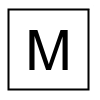
\includegraphics[scale=0.2]{diagrams/overview-presentation/miner-node.png}}}$
			\item Verifier node $\vcenter{\hbox{
\includegraphics[scale=0.2]{diagrams/overview-presentation/verifier-node.png}}}$
		\end{itemize}
	\end{frame}
	
	\begin{frame}
		\frametitle{Design}
		\framesubtitle{Overview}
		\begin{figure}[H]
			\begin{center}
				\resizebox {\columnwidth} {!} {
					\includegraphics<1>{diagrams/overview-presentation/Overview-13.png}
					\includegraphics<2>{diagrams/overview-presentation/Overview-12.png}
					\includegraphics<3>{diagrams/overview-presentation/Overview-11.png}
					\includegraphics<4>{diagrams/overview-presentation/Overview-10.png}
					\includegraphics<5>{diagrams/overview-presentation/Overview-9.png}
					\includegraphics<6>{diagrams/overview-presentation/Overview-8.png}
					\includegraphics<7>{diagrams/overview-presentation/Overview-7.png}
					\includegraphics<8>{diagrams/overview-presentation/Overview-6.png}
					\includegraphics<9>{diagrams/overview-presentation/Overview-5.png}
					\includegraphics<10>{diagrams/overview-presentation/Overview-4.png}
					\includegraphics<11>{diagrams/overview-presentation/Overview-3.png}
					\includegraphics<12>{diagrams/overview-presentation/Overview-2.png}
					\includegraphics<13>{diagrams/overview-presentation/Overview-1.png}
					\includegraphics<14>{diagrams/overview-presentation/Overview-0.png}
			}
			\end{center}
		\end{figure}
	\end{frame}
	
	\begin{frame}
		\frametitle{Design}
		\framesubtitle{Identities}
		Used to anonymously identify a node in a transaction.
		\newline
		
		Balancing goals:
		\begin{itemize}
			\item False location claims must be detectable.
			\item Privacy protecting.
		\end{itemize}
	\end{frame}
	
	\begin{frame}
		\frametitle{Design}
		\framesubtitle{Identities: Nonce Lists}
		\begin{figure}[H]
			\resizebox {\columnwidth} {!} {\begin{tikzpicture}[>=latex]

\tikzset{
mymat/.style={
  matrix of math nodes,
  text height=2.5ex,
  text depth=0.75ex,
  text width=5.25ex,
  align=center,
  column sep=-\pgflinewidth
  },
mymats/.style={
  mymat,
  text width=8ex,
  nodes={draw}
  }  
}

\matrix[mymat,anchor=west,row 1/.style={nodes=draw}]
at (0,0) 
(mat1)
{
\only<1>{4827 & 1928 & 9183}
\only<2->{4827 & 1928 & 9183 & 0047}\\
};
\matrix[mymats=white,anchor=west]
at (0,-3) 
(mat3)
{
\only<-2>{12ef5a1 & c100e9d & 038ef6b}
\only<3->{12ef5a1 & c100e9d & 038ef6b & ee3bc14} \\
};

\node[left=0pt of mat1]
  (cella) {Nonce list:};
  
\node[left=0pt of mat3]
  (cella) {Identities:};
  
\only<3->{ 
\node (key) at ($(mat1-1-4.south)!0.5!(mat3-1-4.north)$) {$K^+(0047)$};
}

\begin{scope}[shorten <= -2pt]
\draw[*->]
  (mat1-1-1.south) -- (mat3-1-1.north);
\draw[*->]
  (mat1-1-2.south) -- (mat3-1-2.north);
\draw[*->]
  (mat1-1-3.south) -- (mat3-1-3.north);
\only<3->{
\draw[*-]
  (mat1-1-4.south) -- (key);
}
\only<3->{
\draw[->]
  (key) -- (mat3-1-4.north);
}
\end{scope}
\end{tikzpicture}}
		\end{figure}
	\end{frame}
	
	\begin{frame}
		\frametitle{Design}
		\framesubtitle{Identities: Duplication}
		Identity duplication is unavoidable in a decentralised system.
		\visible<2->{
		\begin{table}[]
			\begin{tabular}{l|l}
				\textbf{ID} & \textbf{Contents}\\\hline
				\dots & \\\hline
				ffa0 & \\\hline
				ffa1 & \\\hline
				ffa2 & $T_{A4}$ \visible<3->{, \textcolor{red}{$T_{C102}$}}\\\hline
				ffa3 & \\\hline
				ffa4 & $T_{B87}$\\\hline
				\dots & \\
			\end{tabular}
		\end{table}
		}
	\end{frame}
	
	\begin{frame}
		\frametitle{Design}
		\framesubtitle{Transactions}
		Transactions are created when two mobile nodes physically meet.
		\begin{itemize}
			\item Ad-hoc bluetooth connection between the nodes.
		\end{itemize}		
		
		\begin{center}
			\resizebox {0.35\columnwidth} {!} {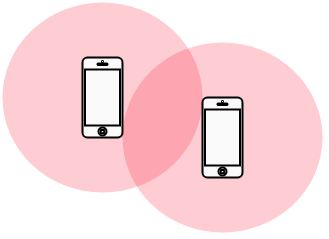
\includegraphics{diagrams/overview-presentation/mobile-node-meet.png}}
		\end{center}
	\end{frame}
	
	\begin{frame}
		\frametitle{Design}
		\framesubtitle{Transactions II}
		Node $A$ will create the following transaction after meeting node $B$:
		\newline
		
		\begin{center}
		\only<1>{$T_{An} = K_A(ts_A|loc_A|ID_{An}|KP_{Bm})$}
		\only<2->{$T_{An} = K_A(ts_A|loc_A|ID_{An}|\textcolor{red}{KP_{Bm}})$}
		\end{center}
	\end{frame}
	
	\begin{frame}
		\frametitle{Design}
		\framesubtitle{Transactions: Key Packets}
		Key Packets provide a Verifier with a means of examining a mobile node's transactions.
		\newline
		
		\only<2->{
		Two main properties:
		\begin{itemize}
			\only<2>{
			\item Allow a Verifier to build a tree of a mobile node's activity.
			}
			\only<3>{
			\item \textcolor{red}{Allow a Verifier to build a graph of a mobile node's activity.}
			}
			\item Allow a mobile node to preserve control its own privacy.
		\end{itemize}
		}
	\end{frame}
	
	\begin{frame}[b]
		\frametitle{Design}
		\framesubtitle{Transactions: Key Packets - Verification}
		\vspace{-0.5cm}
		\begin{figure}
			\resizebox {\columnwidth} {!} {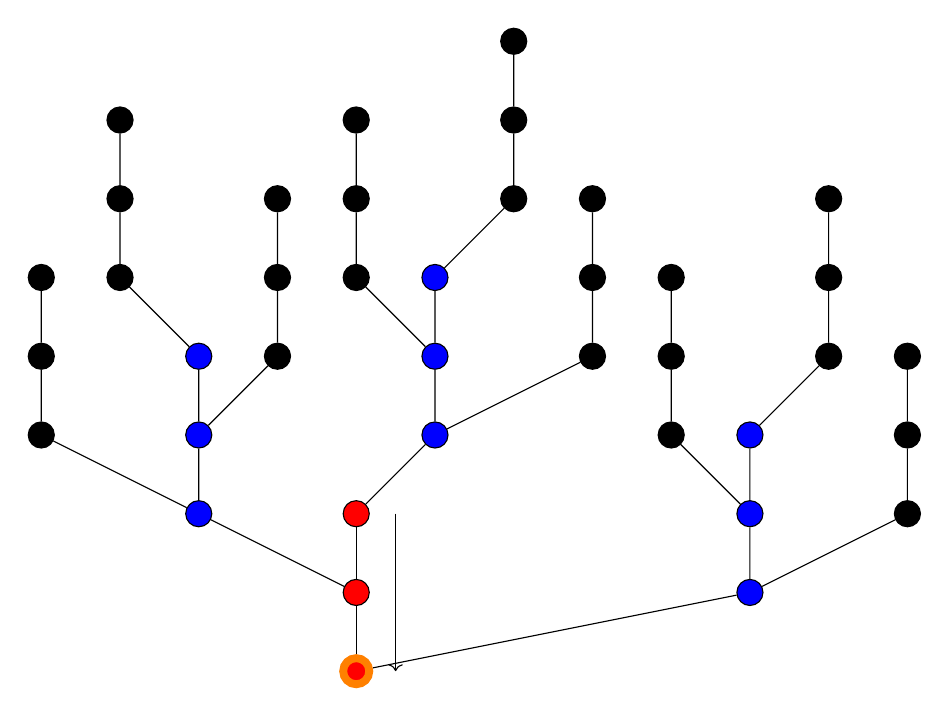
\begin{tikzpicture}[every node/.style={draw,shape=circle,fill=black}]

\node[fill=red,line width=1mm,draw=orange] (A) at (0,0) {};
\node[fill=red] (B) at (0,1) {};
\node[fill=red] (C) at (0,2) {};

\draw (A) -- (B) (B) -- (C);

\only<2> {
\draw[->] (0.5,2) -- (0.5,0);
}

\onslide<3->{
\node[fill=blue] (D) at (5,1) {};
\node[fill=blue] (E) at (5,2) {};
\node[fill=blue] (F) at (5,3) {};

\draw (A) -- (D) (D) -- (E) (E) -- (F);

\node[fill=blue] (G) at (-2,2) {};
\node[fill=blue] (H) at (-2,3) {};
\node[fill=blue] (I) at (-2,4) {};

\draw (B) -- (G) (G) -- (H) (H) -- (I);

\node[fill=blue] (J) at (1,3) {};
\node[fill=blue] (K) at (1,4) {};
\node[fill=blue] (L) at (1,5) {};

\draw (C) -- (J) (J) -- (K) (K) -- (L);
}

\onslide<4->{
\node (M) at (-4,3) {};
\node (N) at (-4,4) {};
\node (O) at (-4,5) {};

\draw (G) -- (M) (M) -- (N) (N) -- (O);

\node (P) at (-1,4) {};
\node (Q) at (-1,5) {};
\node (R) at (-1,6) {};

\draw (H) -- (P) (P) -- (Q) (Q) -- (R);

\node (S) at (-3,5) {};
\node (T) at (-3,6) {};
\node (U) at (-3,7) {};

\draw (I) -- (S) (S) -- (T) (T) -- (U);

\node (V) at (0,5) {};
\node (W) at (0,6) {};
\node (X) at (0,7) {};

\draw (K) -- (V) (V) -- (W) (W) -- (X);

\node (Y) at (2,6) {};
\node (Z) at (2,7) {};
\node (AA) at (2,8) {};

\draw (L) -- (Y) (Y) -- (Z) (Z) -- (AA);

\node (AB) at (3,4) {};
\node (AC) at (3,5) {};
\node (AD) at (3,6) {};

\draw (J) -- (AB) (AB) -- (AC) (AC) -- (AD);

\node (AE) at (4,3) {};
\node (AF) at (4,4) {};
\node (AG) at (4,5) {};

\draw (E) -- (AE) (AE) -- (AF) (AF) -- (AG);

\node (AH) at (6,4) {};
\node (AI) at (6,5) {};
\node (AJ) at (6,6) {};

\draw (F) -- (AH) (AH) -- (AI) (AI) -- (AJ);

\node (AK) at (7,2) {};
\node (AL) at (7,3) {};
\node (AM) at (7,4) {};

\draw (D) -- (AK) (AK) -- (AL) (AL) -- (AM);
}

\end{tikzpicture}}
		\end{figure}
	\end{frame}
	
	\begin{frame}
		\frametitle{Design}
		\framesubtitle{Transactions: Key Packets}
		Key Packets provide a Verifier with a means of examining a mobile node's transactions.
		\newline
		
		Two main properties:
		\begin{itemize}
			\item Allow a Verifier to build a graph of a mobile node's activity.
			\item \textcolor{red}{Allow a mobile node to preserve control its own privacy.}
		\end{itemize}
	\end{frame}
	
	\begin{frame}
		\frametitle{Design}
		\framesubtitle{Transactions: Key Packets - Privacy}
		Published transactions split into two parts: Link and Transaction
		\newline
		
		\begin{figure}
			\resizebox {\columnwidth} {!} {\begin{tikzpicture}[>=latex]

\only<2->{
\node[draw] (A1) at (6,0) {$T_2$};
\node[draw,left=0mm of A1] (A2) {$L_2$};

\only<2>{\node[draw] (B1) at (4,0) {$T_1$};}
\only<3->{\node[draw,fill=gray] (B1) at (4,0) {$T_1$};}
\node[draw,left=0mm of B1] (B2) {$L_1$};

\node[draw] (C1) at (2,0) {$T_0$};
\node[draw,left=0mm of C1] (C2) {$L_0$};

\node (D) at (0.5,0) {$\emptyset$};

\draw[->] ($(A2.west)!0.4!(A2.center)$) -- (B1);
\draw[->] ($(B2.west)!0.4!(B2.center)$) -- (C1);
\draw[->] ($(C2.west)!0.4!(C2.center)$) -- (D);

\onslide<5->{
\node (T) at (6,-1) {\tiny{$KL_{AT}[2]$}};
\node (L) at (5,-1) {\tiny{$KL_{AL}[2]$}};
\draw[->] (L) -- (A2.south);
\draw[->] (T) -- (A1.south);
}

\onslide<6->{
\node (L2) at (3.25,-1) {\tiny{$KL_{AL}[1]$}};
\draw[->] (L2) -- (B2.south);
}
}

\end{tikzpicture}}
		\end{figure}
		\only<4->{
			\begin{center}
				Two \textit{Key Lists}: $KL_{AT}$ and $KL_{AL}$.
			\end{center}
		}
	\end{frame}
	
	\begin{frame}
		\frametitle{Design}
		\framesubtitle{Transactions III}
		Node $A$ will create the following transaction after meeting node $B$:
		
		\begin{center}
		\only<1>{$T_{An} = \textcolor{red}{K_A}(ts_A|loc_A|ID_{An}|KP_{Bm})$}
		\only<2>{$T_{An} = \textcolor{red}{KL_{AT}[n]}(ts_A|loc_A|ID_{An}|KP_{Bm})$}
		\only<3->{$T_{An} = KL_{AT}[n](ts_A|loc_A|ID_{An}|KP_{Bm})$}
		\end{center}
		\vspace{0.5cm}
		
		\only<3->{
		Node $A$ will then publish the following to the blockchain:
		
		\begin{center}
		$P_{An} = ID_{An}|\textcolor{red}{KL_{AL}[n]}(ID_{An-1}|ts_A)|T_{An}$
		\end{center}
		} 
	\end{frame}
	
	\begin{frame}
		\frametitle{Design}
		\framesubtitle{Verification}
		Mobile node needs to provide Verifier node with:
		\begin{itemize}
			\item ID of most recent transaction.
			\item Key Packet for $n$ most recent transactions.
			\item Nonce list for $n$ most recent IDs.
			\item Public key.
		\end{itemize}
	\end{frame}
	
\end{document}